\documentclass[journal,portuguese,english,brazil]{IEEEtran}
%
% If IEEEtran.cls has not been installed into the LaTeX system files,
% manually specify the path to it like:
% \documentclass[journal]{../sty/IEEEtran}
%\usepackage{hyperref}
%\usepackage{breakurl}
\usepackage[portuguese]{babel}
%\usepackage[utf8]{inputenc}
\usepackage[T1]{fontenc}
% Some very useful LaTeX packages include:
% (uncomment the ones you want to load)

\usepackage{breakcites}
\usepackage[hyphens]{url}

\expandafter\def\expandafter\UrlBreaks\expandafter{\UrlBreaks%  save the current one
  \do\a\do\b\do\c\do\d\do\e\do\f\do\g\do\h\do\i\do\j%
  \do\k\do\l\do\m\do\n\do\o\do\p\do\q\do\r\do\s\do\t%
  \do\u\do\v\do\w\do\x\do\y\do\z\do\A\do\B\do\C\do\D%
  \do\E\do\F\do\G\do\H\do\I\do\J\do\K\do\L\do\M\do\N%
  \do\O\do\P\do\Q\do\R\do\S\do\T\do\U\do\V\do\W\do\X%
  \do\Y\do\Z}
  
  \def\UrlBigBreaks{\do\/\do-\do:}

\usepackage[breaklinks=true,colorlinks]{hyperref}
\hypersetup{colorlinks,linkcolor=black,anchorcolor=black,citecolor=black,urlcolor=black}
\usepackage[hyphenbreaks]{breakurl}
\usepackage{lineno}
\modulolinenumbers[5]


% *** MISC UTILITY PACKAGES ***
%
%\usepackage{ifpdf}
% Heiko Oberdiek's ifpdf.sty is very useful if you need conditional
% compilation based on whether the output is pdf or dvi.
% usage:
% \ifpdf
%   % pdf code
% \else
%   % dvi code
% \fi
% The latest version of ifpdf.sty can be obtained from:
% http://www.ctan.org/tex-archive/macros/latex/contrib/oberdiek/
% Also, note that IEEEtran.cls V1.7 and later provides a builtin
% \ifCLASSINFOpdf conditional that works the same way.
% When switching from latex to pdflatex and vice-versa, the compiler may
% have to be run twice to clear warning/error messages.



% *** CITATION PACKAGES ***
%
\usepackage{cite}
% cite.sty was written by Donald Arseneau
% V1.6 and later of IEEEtran pre-defines the format of the cite.sty package
% \cite{} output to follow that of IEEE. Loading the cite package will
% result in citation numbers being automatically sorted and properly
% "compressed/ranged". e.g., [1], [9], [2], [7], [5], [6] without using
% cite.sty will become [1], [2], [5]--[7], [9] using cite.sty. cite.sty's
% \cite will automatically add leading space, if needed. Use cite.sty's
% noadjust option (cite.sty V3.8 and later) if you want to turn this off
% such as if a citation ever needs to be enclosed in parenthesis.
% cite.sty is already installed on most LaTeX systems. Be sure and use
% version 4.0 (2003-05-27) and later if using hyperref.sty. cite.sty does
% not currently provide for hyperlinked citations.
% The latest version can be obtained at:
% http://www.ctan.org/tex-archive/macros/latex/contrib/cite/
% The documentation is contained in the cite.sty file itself.




% *** MATH PACKAGES ***
%
\usepackage[cmex10]{amsmath}
% A popular package from the American Mathematical Society that provides
% many useful and powerful commands for dealing with mathematics. If using
% it, be sure to load this package with the cmex10 option to ensure that
% only type 1 fonts will utilized at all point sizes. Without this option,
% it is possible that some math symbols, particularly those within
% footnotes, will be rendered in bitmap form which will result in a
% document that can not be IEEE Xplore compliant!
%
% Also, note that the amsmath package sets \interdisplaylinepenalty to 10000
% thus preventing page breaks from occurring within multiline equations. Use:
\interdisplaylinepenalty=2500
% after loading amsmath to restore such page breaks as IEEEtran.cls normally
% does. amsmath.sty is already installed on most LaTeX systems. The latest
% version and documentation can be obtained at:
% http://www.ctan.org/tex-archive/macros/latex/required/amslatex/math/





% *** SPECIALIZED LIST PACKAGES ***
%
%\usepackage{algorithmic}
% algorithmic.sty was written by Peter Williams and Rogerio Brito.
% This package provides an algorithmic environment fo describing algorithms.
% You can use the algorithmic environment in-text or within a figure
% environment to provide for a floating algorithm. Do NOT use the algorithm
% floating environment provided by algorithm.sty (by the same authors) or
% algorithm2e.sty (by Christophe Fiorio) as IEEE does not use dedicated
% algorithm float types and packages that provide these will not provide
% correct IEEE style captions. The latest version and documentation of
% algorithmic.sty can be obtained at:
% http://www.ctan.org/tex-archive/macros/latex/contrib/algorithms/
% There is also a support site at:
% http://algorithms.berlios.de/index.html
% Also of interest may be the (relatively newer and more customizable)
% algorithmicx.sty package by Szasz Janos:
% http://www.ctan.org/tex-archive/macros/latex/contrib/algorithmicx/




% *** ALIGNMENT PACKAGES ***
%
\usepackage{array}
% Frank Mittelbach's and David Carlisle's array.sty patches and improves
% the standard LaTeX2e array and tabular environments to provide better
% appearance and additional user controls. As the default LaTeX2e table
% generation code is lacking to the point of almost being broken with
% respect to the quality of the end results, all users are strongly
% advised to use an enhanced (at the very least that provided by array.sty)
% set of table tools. array.sty is already installed on most systems. The
% latest version and documentation can be obtained at:
% http://www.ctan.org/tex-archive/macros/latex/required/tools/


% IEEEtran contains the IEEEeqnarray family of commands that can be used to
% generate multiline equations as well as matrices, tables, etc., of high
% quality.




% *** SUBFIGURE PACKAGES ***
\ifCLASSOPTIONcompsoc
  \usepackage[caption=false,font=normalsize,labelfont=sf,textfont=sf]{subfig}
\else
  \usepackage[caption=false,font=footnotesize]{subfig}
\fi
% subfig.sty, written by Steven Douglas Cochran, is the modern replacement
% for subfigure.sty, the latter of which is no longer maintained and is
% incompatible with some LaTeX packages including fixltx2e. However,
% subfig.sty requires and automatically loads Axel Sommerfeldt's caption.sty
% which will override IEEEtran.cls' handling of captions and this will result
% in non-IEEE style figure/table captions. To prevent this problem, be sure
% and invoke subfig.sty's "caption=false" package option (available since
% subfig.sty version 1.3, 2005/06/28) as this is will preserve IEEEtran.cls
% handling of captions.
% Note that the Computer Society format requires a larger sans serif font
% than the serif footnote size font used in traditional IEEE formatting
% and thus the need to invoke different subfig.sty package options depending
% on whether compsoc mode has been enabled.
%
% The latest version and documentation of subfig.sty can be obtained at:
% http://www.ctan.org/tex-archive/macros/latex/contrib/subfig/




% *** FLOAT PACKAGES ***
%
\usepackage{fixltx2e}
% fixltx2e, the successor to the earlier fix2col.sty, was written by
% Frank Mittelbach and David Carlisle. This package corrects a few problems
% in the LaTeX2e kernel, the most notable of which is that in current
% LaTeX2e releases, the ordering of single and double column floats is not
% guaranteed to be preserved. Thus, an unpatched LaTeX2e can allow a
% single column figure to be placed prior to an earlier double column
% figure. The latest version and documentation can be found at:
% http://www.ctan.org/tex-archive/macros/latex/base/


%\usepackage{stfloats}
% stfloats.sty was written by Sigitas Tolusis. This package gives LaTeX2e
% the ability to do double column floats at the bottom of the page as well
% as the top. (e.g., "\begin{figure*}[!b]" is not normally possible in
% LaTeX2e). It also provides a command:
%\fnbelowfloat
% to enable the placement of footnotes below bottom floats (the standard
% LaTeX2e kernel puts them above bottom floats). This is an invasive package
% which rewrites many portions of the LaTeX2e float routines. It may not work
% with other packages that modify the LaTeX2e float routines. The latest
% version and documentation can be obtained at:
% http://www.ctan.org/tex-archive/macros/latex/contrib/sttools/
% Do not use the stfloats baselinefloat ability as IEEE does not allow
% \baselineskip to stretch. Authors submitting work to the IEEE should note
% that IEEE rarely uses double column equations and that authors should try
% to avoid such use. Do not be tempted to use the cuted.sty or midfloat.sty
% packages (also by Sigitas Tolusis) as IEEE does not format its papers in
% such ways.
% Do not attempt to use stfloats with fixltx2e as they are incompatible.
% Instead, use Morten Hogholm'a dblfloatfix which combines the features
% of both fixltx2e and stfloats:
%
% \usepackage{dblfloatfix}
% The latest version can be found at:
% http://www.ctan.org/tex-archive/macros/latex/contrib/dblfloatfix/




%\ifCLASSOPTIONcaptionsoff
%  \usepackage[nomarkers]{endfloat}
% \let\MYoriglatexcaption\caption
% \renewcommand{\caption}[2][\relax]{\MYoriglatexcaption[#2]{#2}}
%\fi
% endfloat.sty was written by James Darrell McCauley, Jeff Goldberg and 
% Axel Sommerfeldt. This package may be useful when used in conjunction with 
% IEEEtran.cls'  captionsoff option. Some IEEE journals/societies require that
% submissions have lists of figures/tables at the end of the paper and that
% figures/tables without any captions are placed on a page by themselves at
% the end of the document. If needed, the draftcls IEEEtran class option or
% \CLASSINPUTbaselinestretch interface can be used to increase the line
% spacing as well. Be sure and use the nomarkers option of endfloat to
% prevent endfloat from "marking" where the figures would have been placed
% in the text. The two hack lines of code above are a slight modification of
% that suggested by in the endfloat docs (section 8.4.1) to ensure that
% the full captions always appear in the list of figures/tables - even if
% the user used the short optional argument of \caption[]{}.
% IEEE papers do not typically make use of \caption[]'s optional argument,
% so this should not be an issue. A similar trick can be used to disable
% captions of packages such as subfig.sty that lack options to turn off
% the subcaptions:
% For subfig.sty:
% \let\MYorigsubfloat\subfloat
% \renewcommand{\subfloat}[2][\relax]{\MYorigsubfloat[]{#2}}
% However, the above trick will not work if both optional arguments of
% the \subfloat command are used. Furthermore, there needs to be a
% description of each subfigure *somewhere* and endfloat does not add
% subfigure captions to its list of figures. Thus, the best approach is to
% avoid the use of subfigure captions (many IEEE journals avoid them anyway)
% and instead reference/explain all the subfigures within the main caption.
% The latest version of endfloat.sty and its documentation can obtained at:
% http://www.ctan.org/tex-archive/macros/latex/contrib/endfloat/
%
% The IEEEtran \ifCLASSOPTIONcaptionsoff conditional can also be used
% later in the document, say, to conditionally put the References on a 
% page by themselves.




% *** PDF, URL AND HYPERLINK PACKAGES ***
%
\usepackage{url}
% url.sty was written by Donald Arseneau. It provides better support for
% handling and breaking URLs. url.sty is already installed on most LaTeX
% systems. The latest version and documentation can be obtained at:
% http://www.ctan.org/tex-archive/macros/latex/contrib/url/
% Basically, \url{my_url_here}.




% *** Do not adjust lengths that control margins, column widths, etc. ***
% *** Do not use packages that alter fonts (such as pslatex).         ***
% There should be no need to do such things with IEEEtran.cls V1.6 and later.
% (Unless specifically asked to do so by the journal or conference you plan
% to submit to, of course. )

\title{\LARGE \bf
A Survey On Visible Light Positioning And Its Applications For Autonomous Mobility
}

\author{Mateus Rodrigues Santos, Danilo Alves de Lima, Arthur de Miranda Neto % <-this % stops a space
\thanks{The authors are with Terrestrial Mobility Lab. at the Federal University of Lavras (UFLA), Brazil. During this study, M. R. Santos was supported by a scholarship from CNPq/Brazil. A. Miranda Neto is projects coordinator of 88881.067959/2014-01 and 88881.068069/2014-01 from CAPES/Brazil. Contact the authors: {\tt \{santos.mrodrigues0\}@gmail.com} and {\tt \{danilo.delima, arthur.miranda\}@deg.ufla.br}.}
}

\begin{document}
\selectlanguage{brazil}
%\newcounter{mytempeqncnt}

\maketitle
\thispagestyle{empty}
\pagestyle{empty}

%%%%%%%%%%%%%%%%%%%%%%%%%%%%%%%%%%%%%%%%%%%%%%%%%%%%%%%%%%%%%%%%%%%%%%%%%%%%%%%%
\begin{abstract}

The rise of technologies in the field of autonomous mobility has allowed, recently, a great advance in relation to the level of automation of intelligent vehicles. However, there are several elements to be improved in order to have these vehicles on road. One of them is the global positioning at low cost. In this scope, this study is a survey on Visible Light Positioning techniques with the objective of tracing the state of the art on this technology, searching applicability to the field of autonomous mobility, in order to overcome the positioning barrier. The results catalogued from the literature on the actual scenario justify the application proposal. 

\end{abstract}

\begin{IEEEkeywords}
Localization, Visible Light Communication and Positioning, Signal Processing, Intelligent Vehicles.
\end{IEEEkeywords}
%%%%%%%%%%%%%%%%%%%%%%%%%%%%%%%%%%%%%%%%%%%%%%%%%%%%%%%%%%%%%%%%%%%%%%%%%%%%%%%%
\nopagebreak
\section{Introdu��o} \label{sec:introduction}

\IEEEPARstart{S}{istemas} de posicionamento s�o aqueles usados para se obter o posicionamento de objetos no espa�o por meio de uma s�rie de t�cnicas que variam de acordo com o prop�sito da aplica��o. A tecnologia mais comum utilizada, hodiernamente, ainda � o Sistema de Posicionamento Global (GPS - \textit{Global Positioning System}). Entretanto, novas aplica��es v�m requerendo novas tecnologias que aumentam a precis�o e reduzam problemas atrelados aos GPS, tais como a perda de sinal em ambientes internos e a grande interfer�ncia em abientes urbanos com alta densidade de edifica��es. A busca por tecnologias que aperfei�oem sistemas de posicionamento se faz de grande import�ncia para a mobilidade aut�noma no cen�rio atual de desenvolvimento. As tecnologias alternativas principais, em estudo, s�o diversas, como a localiza��o via frequ�ncias de R�dio; via wi-fi, e a que se faz objeto de estudo deste trabalho, Comunica��o por meio da Luz Vis�vel (VLC - \textit{Visible Light Communication})~\cite{7781952,7737307}.

No contexto da VLC, � importante remeter � ascens�o	de tecnologias nos dispositivos de ilumina��o de estado s�lido (SSL - \textit{Solid State Lightning}) como os Diodos Emissores de Luz (LED - \textit{Light Emmiting Diode}) e sua populariza��o na ilumina��o artificial em v�rios n�veis, desde residencial � p�blica. Isto se deve principalmente � sua alta efici�ncia (200\% de ilumina��o por unidade de consumo de energia em rela��o �s l�mpadas fluorescentes), alta durabilidade (500\% em rela��o �s fluorescentes), e um baixo custo de implementa��o. Essa populariza��o rendeu a descoberta de m�todos de comunica��o n�o conhecidos antes. A partir da utiliza��o de fotodetectores (sensores de luz, fotodiodos, fototransistores, entre outros) ou sensores de imagem (c�meras fotogr�ficas), s�o estudadas t�cnicas de transmiss�o de dados que superam a velocidade de transmiss�o por ondas de r�dio, atualmente amplamente utilizada para comunica��es. � v�lido ressaltar que os sistemas citados cumprem o objetivo de ilumina��o tanto quanto de transmiss�o de dados~\cite{7239528}.

Atrelado ao desenvolvimento da tecnologia de VLC, est� o Posicionamento por meio da Luz Vis�vel (VLP - \textit{Visible Light Positioning.}), tecnologia que consiste no uso de t�cnicas, baseadas em VLC, para o posicionamento refereciado de objetos. As t�cnicas de comunica��o, em conjunto com um processamento de sinais espec�fico para o posicionamento, permitem que um sistema seja capaz de calcular sua localiza��o espacial a partir de diferentes fontes de luz. A tecnologia fornece, segundo resultados obtidos at� ent�o, sistemas robustos e vers�teis que resolvem os principais problemas da utiliza��o de GPS; a literatura prev� posicionamentos at� 20 vezes mais precisos que os sistemas de GPS convencionais e sistemas que atendem a ambientes urbanos e principalmente a ambientes internos. O objetivo desse estudo �, ent�o, modelar o funcionamento b�sico dos sistemas de VLP para analisar suas principais t�cnicas e tra�ar um comparativo destas com base nos resultados encontrados at� ent�o na literatura, analisando os sistemas quanto � sua robustez e aplicabilidade.


\input{Comunicacao}
\section{Posicionamento por meio da Luz Vis�vel} \label{sec:posicionamento}

S�o tr�s os principais par�metros de um sistema de VLP a se considerar para o entendimento do modelo b�sico: o transmissor, o receptor e o ambiente. Eles est�o simplificados na Figura~\ref{fig:2}, em que est� ilustrado o funcionamento b�sico da camada f�sica. Importante considerar que a luz emitida tra�a basicamente dois tipos de caminho para alcan�ar o receptor, um caminho direto (LOS - \textit{Line-of-Sigh}), e um caminho indireto (NLOS - \textit{Non-Line-of-Sigh.}), proveniente dos sinais luminosos refletidos nas paredes ou obst�culos. As dimens�es e geometrias do ambiente determinam o modelo para cada um dos sinais recebidos. Entretanto, a influ�ncia dos sinais NLOS para sistemas de baixa taxa de transmiss�o de dados, como os de posicionamento, � desprez�vel~\cite{yan2015current}. Neste sistema, a pot�ncia do sinal �ptico recebida no sensor ($P_{R}$) pode ser modelada pela equa��o 1, que leva em considera��o a pot�ncia luminosa emitida ($P_{T}$), a dist�ncia entre transmissor e emissor ($d$), o padr�o de radia��o do emissor de luz em fun��o do �ngulo de irradia��o ($R_{E}(\phi)$), filtros �pticos ($T(\psi)$)(implementados no hardware do receptor), concentradores �pticos ($G(\psi)$)(lentes), a �rea f�sica do receptor ($A_{R}$), e por fim o �ngulo de incid�ncia do sinal luminoso ($cos(\psi)$)~\cite{de2015test}.
%
\begin{figure}[!h]
    \centering
    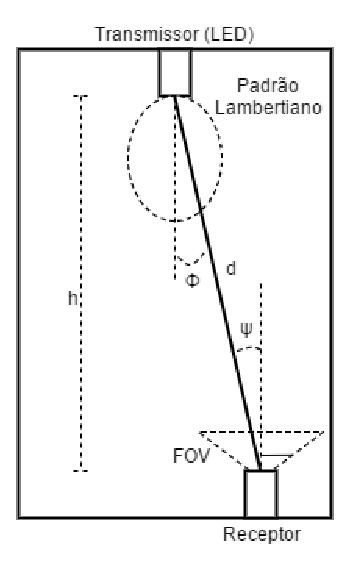
\includegraphics{FIGURA2}
    \caption[Esquem�tico b�sico de sistema de VLP considerando um receptor �nico, um transmissor LED e os par�metros espaciais supracitados. A imagem ilustra, tamb�m, o padr�o Lambertiano de irradia��o e o campo de vis�o de incid�ncia (FOV - \textit{Field of View}).]{Esquem�tico b�sico de sistema de VLP considerando um receptor �nico, um transmissor LED e os par�metros espaciais supracitados. A imagem ilustra, tamb�m, o padr�o Lambertiano de irradia��o e o campo de vis�o de incid�ncia (FOV - \textit{Field of View}).\footnotemark}
    \label{fig:2}
\end{figure}
    \footnotetext{O padr�o lambertiano � caracter�stica intr�nseca de um LED de superf�cie emissora, e tem rela��o direta com a �rea efetiva de ilumina��o do LED. Este padr�o modela o comportamento da pot�ncia de sinal incidido em fun��o do �ngulo $\phi$ em rela��o � normal do LED~\cite{keiser2014comunicaccoes}.}
%    
\begin{equation}
P_{R} = \frac{P_{T}}{d^2} R_{E} (\phi) T (\psi) G (\psi) A_{R} cos (\psi).
\end{equation}

Neste modelo, as fun��es do campo de vis�o podem ser sintetizadas em apenas um par�metro, chamado �rea efetiva de recep��o de sinais ($A_{ef} (\psi)$) (Equa��o 2), dependente das caracter�sticas do sensor utilizado e da implementa��o ou n�o de filtros e concentradores �pticos. Enquanto RE � fun��o do padr�o lambertiano do LED utilizado no sistema (Equa��o 3, 4).
%
\begin{equation}
A_{ef} (\psi) = A_{R} cos (\psi) T (\psi) G (\psi).
\end{equation}
%
\begin{equation}
R_{E} (\phi) = \frac{m + 1}{2 \pi} cos^m (\phi).
\end{equation}

\noindent onde m � a ordem lambertiana, dependente do semi�ngulo de emiss�o ($\varphi_{1 / 2}$) (par�metro do LED), definido por:~\cite{de2015test,kim2013indoor}
%
\begin{equation}
m = \frac{-ln (2)}{ln ( cos (\phi_\frac{1}{2} ) )}.
\end{equation}

O conhecimento do comportamento de tais par�metros se faz de suma import�ncia, como se observa nos m�todos de VLP mais relevantes, encontrados na literatura, utilizarem principalmente a amplitude do sinal recebido como par�metro principal nos algoritmos de posicionamento, conforme ser� abordado adiante. Nesse contexto, a Figura~\ref{fig:3} ilustra o comportamento da amplitude normalizada do sinal recebido em fun��o da varia��o de cada par�metro espacial individualmente.
%
\begin{figure*}[tb]
    \centering
    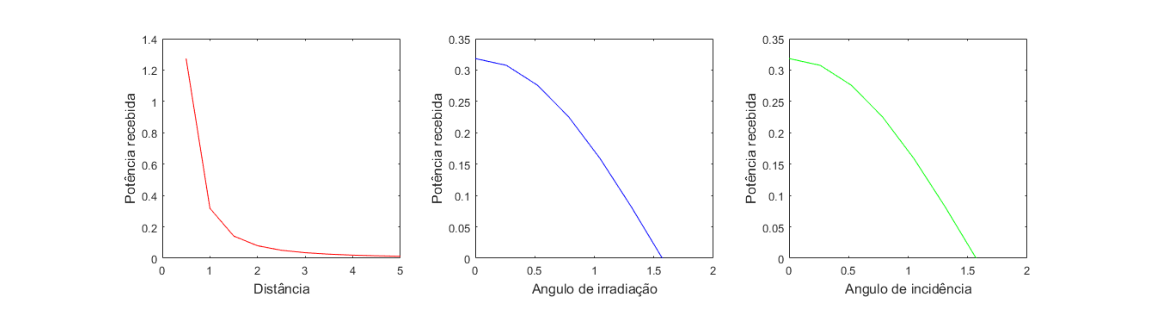
\includegraphics[width = 17 cm]{FIGURA3}
    \caption{Comportamento da amplitude em fun��o da varia��o a) da dist�ncia (d); b) do angulo de incid�ncia ($\psi$); e do �ngulo de irradia��o ($\phi$).}
    \label{fig:3}
\end{figure*}

\subsection{M�todos de Posicionamento}

Diferentes t�cnicas s�o estudadas para o processamento dos sinais recebidos de diversas fontes de luz visando o c�lculo da posi��o do receptor conhecendo a posi��o dos emissores, sendo esse receptor um sensor �nico ou sensor de imagem (composto por uma matriz de sensores de fotodiodos). As quatro principais t�cnicas\footnote{Na literatura mais recente~\cite{7737307}, encontra-se essa divis�o pela tecnologia de comunica��o do canal �ptico; diferindo-se de produ��es anteriores que classificavam pelo m�todo de processamento de sinais~\cite{yan2015current}.} ser�o aprofundadas para posterior compara��o dos resultados obtidos com sua utiliza��o, sendo elas: Divis�o Espacial (SDMA), Divis�o Temporal (TDMA), Divis�o de Frequ�ncias (FDMA), Divis�o de C�digo (CDMA)\footnote{Aqui considera-se apenas as tecnologias de acesso m�ltiplo, desconsiderando o m�todo de proximidade, o qual consiste na detec��o de uma s�rie de pontos de refer�ncia em uma rede e o posicionamento por detec��o desses pontos, devido a sua limita��o de precis�o na resolu��o da rede de transmissores~\cite{chunyue2015research,lee2012hybrid}, o que inviabiliza a an�lise do m�todo para a aplica��o em estudo. As siglas s�o padronizadas com base em~\cite{7737307}, sendo tradu��o para Space Division Multiple Access, Time Division Multiple Access, Frequency Division Multiple Access e CodeDivisionMultiple Access, respectivamente.}.

\subsubsection{Divis�o Espacial}

S�o classificadas como SDMA as t�cnicas de posicionamento em que as informa��es de cada LED s�o recebidas por partes diferentes do sensor. Ou seja, demandam a utiliza��o de sensores de imagem. Seu princ�pio de funcionamento consiste na modula��o dos LEDs em frequ�ncias espec�ficas e aquisi��o de imagens por meio dos sensores, tamb�m em uma dada frequ�ncia. Dessa forma, as imagens s�o processadas para a determina��o de sinais luminosos em certas posi��es e da presen�a de determinadas frequ�ncias. As imagens s�o decodificadas para se obter a localiza��o dos sinais luminosos. No servidor de processamento deve conter um banco de dados com as coordenadas espaciais relacionadas � frequ�ncia emitida por cada LED. Uma vez que os sinais s�o identificados, algoritmos de localiza��o, como por exemplo �ngulo de Aquisi��o (AoA - \textit{Angle of Arrival}) determinam a posi��o do dispositivo receptor~\cite{rahman2011high,kuo2014luxapose}.

A frequ�ncia de amostragem e a capacidade de processamento de imagens dos dispositivos s�o as principais dificuldades da t�cnica em quest�o. C�meras de vis�o computacional convencionais variam sua taxa de aquisi��o de 30 fps a 120 fps, o sendo baixa para a an�lise das frequ�ncias emitidas pelos LEDs. Solu��es tais como a utiliza��o de c�meras de alta velocidade, aumento da densidade de emissores de luz por �rea abrangida, e implementa��o de lentes especiais s�o estudadas na literatura, entretanto aumentam significativamente o custo de implementa��o dessa tecnologia~\cite{7737307,nakazawa2013indoor,kuo2014luxapose}.

\subsubsection{Divis�o Temporal}

Destoante do m�todo supracitado, a divis�o por tempo depende da utiliza��o de apenas um fotosensor na recep��o do sinal. A t�cnica se baseia em cada LED enviar um �nico pulso de sinal sequencialmente para um dado montante de LEDs que cobrem a mesma �rea. Cada pulso � enviado com a mesma largura. Dessa forma, o receptor, ap�s um dado per�odo de tempo, adquire sinais de todos os LEDs da �rea coberta e assimila a pot�ncia do sinal recebido de cada transmissor pela posi��o do pulso no per�odo de tempo.  � importante ressaltar que os demais LEDs do painel, enquanto n�o est�o transmitindo seu sinal, permanecem desligados~\cite{do2014tdoa}, ao menos que seja aplicada uma detec��o de colis�es no sistema~\cite{li2014epsilon}.

A utiliza��o dessa t�cnica acarreta algumas desvantagens ao sistema a exemplo a limita��o na taxa de transmiss�o de dados devido � cada transmissor ser capaz de enviar os dados em um pequeno per�odo de tempo, o que causa uma baixa taxa de atualiza��o no posicionamento de um receptor em movimento. Outra desvantagem relevante � a necessidade de sincronismo do sistema, o que acarreta maior custo de implementa��o e limita��o de acessibilidade dos dispositivos.

Na literatura s�o encontradas implementa��es por divis�o temporal que baseia o processamento dos sinais recebidos principalmente em RSS ou em tempo de chegada (ToA - \textit{Time of Arrival}). Simula��es\footnote{Simula��es no software MATLAB que forneceram resultado de 3,9 cm de erro m�ximo em um ambiente de 5x5x3 m (Dimensionamento m�dio de uma sala residencial).} estimam que o segundo m�todo possa atingir precis�es maiores que a maioria dos sistemas de VLP existentes. Entretanto este requer que o receptor porte de um temporizador altamente preciso, devido � pequena dist�ncia entre os dispositivos transmissores e receptores face � velocidade da luz~\cite{do2014tdoa,7737307}.

\subsubsection{Divis�o de Frequ�ncia}

Ainda sobre a perspectiva de utiliza��o de um receptor �nico, visando alternativas que eliminem a necessidade de sincroniza��o dos transmissores, a tecnologia de FDMA consiste na associa��o de diferentes frequ�ncias a cada LED e processamento dos sinais no dom�nio da frequ�ncia, com a aplica��o de FFT no sinal recebido, e cada transmissor pode ser distinguido pelo espectro transmitido. Devido a n�o sincroniza��o dos dispositivos, o processamento de sinais tem que ser feito por an�lise de pot�ncia do sinal �ptico. A independ�ncia de sincroniza��o, somada � baixa complexidade necess�ria no circuito transmissor tornam esse um m�todo com baixo custo de implementa��o\footnote{Apesar da desvantagem pela perca de efici�ncia m�xima dos dispositivos de LED com a utiliza��o de controladores anal�gicos.}.

Para o entendimento das limita��es da t�cnica � importante retomar a equa��o 1, levando em conta que o processamento dos sinais � feito por meio da pot�ncia do sinal �ptico. A obten��o de informa��o de dist�ncia em fun��o da pot�ncia do sinal de dada frequ�ncia, ou seja, do sinal associado a um LED, � dependente do �ngulo de incid�ncia e do �ngulo de irradia��o, que em um sistema pr�tico dependem da posi��o do transmissor e do receptor, e s�o par�metros n�o fixos. As formas encontradas na literatura para minimizar poss�veis erros gerados na rela��o desses par�metros � a introdu��o de um fator de corre��o encontrando os �ngulos $\phi$ e $\psi$, ou ainda assumindo um sistema onde o transmissor e receptor est�o sempre paralelos e em altura fixa, o que simplifica a equa��o em:
%
\begin{equation}
d = \sqrt[4]{\frac{P_{T} h^2 A_{R}}{P_{R} \pi}}
\end{equation}

\subsubsection{Divis�o de C�digo}

Tecnologia que se baseia na transmiss�o de uma �nica sequ�ncia de informa��es codificadas (digitais) por cada LED. Apesar da transmiss�o de dados, o sistema independe de sincroniza��o, devido � caracter�stica do receptor de conhecer todos os c�digos utilizados em determinada �rea, obtendo-se informa��es de cada LED.
Comumente, essa tecnologia se associa, tamb�m, � utiliza��o da pot�ncia �ptica no algoritmo de posicionamento. No entanto na utiliza��o dessa t�cnica em sistemas de CDMA, atrasos aleat�rios entre os sinais geram grande montante de interfer�ncia de acesso m�ltiplo que influenciam no erro de posicionamento.

Um importante ponto a se considerar nas t�cnicas de CDMA � a influ�ncia negativa na fun��o de ilumina��o dependendo do padr�o de codifica��o utilizado. A maneira de contornar � a padroniza��o dos c�digos de comunica��o para m�todos que definem a pot�ncia m�dia de sa�da nos LEDs, tais como c�digos de comunica��o por r�dio frequ�ncia (RF - \textit{Radio Frequency}), que tem uma pot�ncia de sa�da m�dia de 50\%~\cite{7737307}.

\subsection{O Estado da Arte} \label{estadodaarte}

No contexto desta tecnologia em ascens�o, diversos m�todos t�m sido estudados visando � viabiliza��o e aplica��o da VLP\footnote{Principalmente para o posicionamento em ambientes internos e para a mobilidade urbana.}. Frente a este cen�rio, resultados variados demonstram a evolu��o atual permitindo entender as perspectivas deste campo de estudo.  A Tabela~\ref{tab:1}, anexada ao final deste texto, exp�e os resultados mais relevantes encontrados na literatura, em fun��o do m�todo de posicionamento utilizado, a �rea abrangida pelo sistema, o erro associado ao posicionamento, e as principais caracter�sticas individuais de cada um.
%
\begin{table}[tb]
\centering
\caption{O Estado da Arte}
\label{tab:1}
\resizebox{\textwidth}{!}{%
\begin{tabular}{|l|l|l|l|c|}
\hline
\multicolumn{1}{|c|}{\textbf{\begin{tabular}[c]{@{}c@{}}Pesquisador\end{tabular}}} & \multicolumn{1}{c|}{\textbf{\begin{tabular}[c]{@{}c@{}}T�cnica de\\   VLP\end{tabular}}} & \multicolumn{1}{c|}{\textbf{\begin{tabular}[c]{@{}c@{}}Alcance de\\   opera��o (m)\end{tabular}}} & \multicolumn{1}{c|}{\textbf{\begin{tabular}[c]{@{}c@{}}Precis�o\\   Obtida\end{tabular}}} & \textbf{\begin{tabular}[c]{@{}c@{}}Caracter�sticas\\   (m�todo de medi��o, sincronismo, custo, caracter�sticas individuais)\end{tabular}} \\ \hline
\textbf{~\cite{nadeem2014highly}} & TDMA & 5x5x3 & 1mm & \begin{tabular}[c]{@{}c@{}}TDoA, sistema de transmiss�o sincronizado, baixo custo de\\   implementa��o, resultados de simula��o, posicionamento tridimensional\end{tabular} \\ \hline
\textbf{~\cite{de2015test}} & CDMA & 3x3x2 & 0.7 m & \begin{tabular}[c]{@{}c@{}}RSSI,\\   sistema n�o sincronizado, baixo custo, resultados experimentais, o acesso\\   m�ltiplo aumenta o erro de posicionamento.\end{tabular} \\ \hline
\textbf{~\cite{yang2014three}} & CDMA & 2 x 2 x 2.5 & 2.3cm & \begin{tabular}[c]{@{}c@{}}AoA e RSSI, sistema n�o sincronizado, baixo custo, resultados de\\   simula��o, utiliza��o de um �nico transmissor e m�ltiplos receptores,\\   posicionamento tridimensional\end{tabular} \\ \hline
\textbf{~\cite{kuo2014luxapose}} & SDMA & 0.71 x 0.73 & 0.1 m & \begin{tabular}[c]{@{}c@{}}AoA,\\   sistema n�o sincronizado, baixo custo, resultados experimentais, capacidade\\   de estimar orienta��o do receptor\end{tabular} \\ \hline
\textbf{~\cite{kim2013indoor}} & FDMA & 1 x 1 x 0.6 & 0.2 cm 2.4 cm & RSSI, sistema n�o sincronizado, baixo custo, resultados experimentais. \\ \hline
\textbf{~\cite{li2014epsilon}} & FDMA & 20 x 20 x 3 & <O.4 m & \begin{tabular}[c]{@{}c@{}}RSSI,\\   transmiss�o de dados n�o sincronizada, baixo custo de implementa��o,\\   resultados de simula��o\end{tabular} \\ \hline
\textbf{~\cite{sahin2015accuracy}} & TDMA & 3 x 5 x 4 & < 1 m & \begin{tabular}[c]{@{}c@{}}AoA e RSS, sistema previsto em modelo matem�tico, sem previs�o de\\   implementa��o\end{tabular} \\ \hline
\textbf{~\cite{qiu2015visible}} & SDMA & 4.7 x 8.6 & 0.56 m & \begin{tabular}[c]{@{}c@{}}Infer�ncia\\   Gaussiana e Bayesiana, sistema n�o sincronizado, baixo custo, resultados\\   experimentais,\end{tabular} \\ \hline
\textbf{~\cite{luo2013indoor}} & FDMA & 2x2x2 & 18mm & \begin{tabular}[c]{@{}c@{}}RSSI, sistema de transmiss�o n�o sincronizado, baixo custo de\\   implementa��o, resultados de simula��o, sistema com transmiss�o de dados em\\   alta frequ�ncia dento da baixa frequ�ncia utilizada para o posicionamento.\\   Constata��o de diminui��o do erro de posicionamento em dez vezes a cada 10 dB\\   aumentados na rela��o sinal/ru�do.\end{tabular} \\ \hline
\textbf{~\cite{do2014tdoa}} & TDMA & 5x5x3 & 3,9 cm & \begin{tabular}[c]{@{}c@{}}TDoA,\\   sistema de transmiss�o sincronizado, alto custo de implementa��o, resultados\\   de simula��o usando MATLAB\end{tabular} \\ \hline
\textbf{~\cite{rahman2011high}} & SDMA & 1,8x1,8x3,5 & 10 cm & \begin{tabular}[c]{@{}c@{}}Processamento de imagem, sistema n�o sincronizado, sem par�metro de\\   custo, resultados de simula��es, o sistema tem suas vantagens na simplicidade\\   e independ�ncia de refer�ncias angulares.\end{tabular} \\ \hline
\textbf{~\cite{kail2014robust}} & CDMA & 30x30x4 & 0,81m & \begin{tabular}[c]{@{}c@{}}Infer�ncia\\   Bayesiana, sem necessidade de sincroniza��o, baixo custo de implementa��o,\\   resultados de simula��o com MATLAB, considera funcionamento com influ�ncia de\\   NLOS\end{tabular} \\ \hline
\textbf{~\cite{yi2015development}} & TDMA & 1,2x1,2x1,7 & 3cm & \begin{tabular}[c]{@{}c@{}}RSSI, sistema sincronizado, baixo custo de implementa��o,utiliza��o de\\   bit stuffing para otimiza��o do sistema de VLC, aplica��o em rob�tica m�vel\end{tabular} \\ \hline
\textbf{~\cite{jung2014indoor}} & TDMA & 1,0x1,0x1,3 & 3,24cm & \begin{tabular}[c]{@{}c@{}}RSSI,\\   sistema sincronizado, alto custo, necess�rio que a altura do receptor seja\\   fixa e conhecida\end{tabular} \\ \hline
\textbf{~\cite{yamaguchi2014design}} & CDMA & 6x6x0,4 & 8cm & \begin{tabular}[c]{@{}c@{}}OOC, sistema n�o sincronizado, baixo custo, resultados dados por\\   simula��o e modelo matem�tico, combina��o de transmiss�o de dados para cobertura\\   de �reas maiores\end{tabular} \\ \hline
\textbf{~\cite{moon2014indoor}} & SDMA & 1,8x1,8x3,5 & 0,09x0,08x0,44 cm & \begin{tabular}[c]{@{}c@{}}Processamento\\   de imagem, sistema n�o sincronizado, sem par�metro de custo, resultados por\\   simula��o, posicionamento tri dimensional.\end{tabular} \\ \hline
\textbf{~\cite{yasir2014indoor}} & TDMA & 5x3x3 & 25cm & \begin{tabular}[c]{@{}c@{}}RSSI, sistema sincronizado, baixo custo, resultados experimentais, sensoriamento\\   h�brido com o uso de sensores inerciais, posicionamento tri dimensional\end{tabular} \\ \hline
\textbf{~\cite{zhang2014asynchronous}} & TDMA & 6x6x4 & 11,2cm & \begin{tabular}[c]{@{}c@{}}RSSI e\\   ToA, sistema n�o sincronizado com detector de colis�o, baixo custo, receptor\\   em altura fixa e conhecida, resultados de simula��o\end{tabular} \\ \hline
\textbf{~\cite{nakazawa2013indoor}} & SDMA & 7,5x5,4x3 & 10cm & \begin{tabular}[c]{@{}c@{}}Processamento de imagem, sistema sincronizado, alto custo, resultados\\   experimentais, utiliza��o de lente olho de peixe para melhoria do\\   posicionamento por abranger mais transmissores no FOV de recep��o.\end{tabular} \\ \hline
\textbf{~\cite{zhang2014theoretical}} & FDMA & 2,2x2,2x3 & - & \begin{tabular}[c]{@{}c@{}}RSSI,\\   sistema n�o sincronizado, baixo custo, teste da influ�ncia de diversos\\   par�metros do modelo de RSSI para VLP no erro de posicionamento por meio de\\   simula��es.\end{tabular} \\ \hline
\textbf{~\cite{kim2016vehicle}} & SDMA & 20x6x5 & 1m & \begin{tabular}[c]{@{}c@{}}Processamento de imagem, sistema n�o sincronizado, baixo custo,\\   resultados de simula��o, aplica��o para mobilidade terrestre.\end{tabular} \\ \hline
\textbf{~\cite{hu2016demonstration}} & TDMA & 2,5x2,5x2 & 10cm & \begin{tabular}[c]{@{}c@{}}RSSI,\\   sistema sincronizado, baixo custo, resultados experimentais, aplica��o para\\   rob�tica m�vel.\end{tabular} \\ \hline
\textbf{~\cite{see2016investigation}} & FDMA & 0,95x0,9x0,6 & 40cm & \begin{tabular}[c]{@{}c@{}}RSSI, sistema n�o sincronizado, baixo custo, resultados experimentais,\\   sistema de baixa complexidade.\end{tabular} \\ \hline
\textbf{~\cite{7781952}} & CDMA & 20x20x5 & <60cm & \begin{tabular}[c]{@{}c@{}}Estima��o\\   de par�metros, sistema n�o sincronizado, baixo custo, resultados de simula��o\\   com transmissores espalhados em forma de domo.\end{tabular} \\ \hline
\end{tabular}%
}
\end{table}
\section{Aplica��es para a Mobilidade Aut�noma}

Atrelado ao atual desenvolvimento no campo da mobilidade aut�noma e ao crescente n�vel de automa��o dos ve�culos que comp�e o mercado, algumas limita��es ainda s�o inerentes aos sistemas de intelig�ncia veicular. No �mbito do posicionamento global, par�metro fundamental para todo n�vel de automa��o veicular, a limita��o se encontra nos sistemas de posicionamento global tradicionais (GPS), os quais n�o fornecem precis�o suficiente para garantir a seguran�a, e tem seu funcionamento limitado em �reas urbanas~\cite{kim2016vehicle}.

Esse cen�rio converge na busca por m�todos alternativos que viabilizem a localiza��o precisa nesses ambientes. O VLP se mostra como solu��o atrativa, visto a jun��o de um posicionamento local relativamente preciso, em grande parte dos resultados para posicionamento em grandes �reas\footnote{Com grandes �reas, entende-se de tamanho suficiente para o posicionamento de um ve�culo baseado na utiliza��o de l�mpadas de ilumina��o p�blica.}, e o baixo custo de implementa��o, face � possibilidade de utiliza��o da pr�pria infraestrutura de ilumina��o p�blica. 

A limita��o primordial de tal aplica��o � referente � ampla gama de interfer�ncia nos sistemas, devido a se colocarem em ambiente aberto, sujeito � luz solar e outras fontes de ilumina��o artificial. Esse se mostra como grande desafio a ser superado na literatura\footnote{Neste ponto, justificam-se as principais vantagens da aplica��o de t�cnicas de FDMA, devido � sua robustez frente a interfer�ncias externas.}.
Outro fator relevante � aplicabilidade da tecnologia rememora o fato de ve�culos tamb�m possu�rem dispositivos luminosos, possibilitando a comunica��o n�o apenas no sentido infraestrutura para ve�culos (I2V), mas tamb�m de ve�culos para infraestrutura (V2I) e ve�culos para ve�culos (V2V). Ainda � importante ressaltar a acessibilidade urbana atrelada � aplica��o de VLC sendo disponibilizada na ilumina��o p�blica, contribuindo, em an�lise ampla, ao desenvolvimento das cidades inteligentes~\cite{7239528,do2016visible}.

\section{Considera��es Finais} 

Tendo por base os resultados catalogados no item~\ref{estadodaarte}, observa-se o potencial das tecnologias ascendentes de posicionamento com base em VLC. Conforme supracitado, o emprego destas nos campos da mobilidade urbana. Resultados mais promissores demonstram precis�es de 0,1 a 1 metro para �reas aplic�veis ao ambiente urbano, atrelando robustez e baixo custo em sua implementa��o. Nesse trabalho, conclui-se que a alternativa proposta se demonstra como alternativa plaus�vel e a ser amplamente estudada para contribui��o no desenvolvimento de ve�culos inteligentes. 

Como perspectiva futura, pretende-se validar os m�todos estudados para VLP por meio da obten��o de resultados pr�prios, com foco no estudo de FDMA, e a implementa��o em m�dio-longo prazo de testes da tecnologia para ve�culos inteligentes.

%\section*{Acknowledgement}

%This study was carried out and funded in the framework of the Equipex ROBOTEX (Reference ANR-10-EQPX-44-01). It was equally supported by the French Picardie project VERVE, French Government, through the program ``Investments for the future" managed by the National Agency for Research, and the the European Fund of Regional Development FEDER. The authors wish to thank the helpful assistance of G\'{e}rald Dherbomez, Giovani B. Vitor, Pierre Hudelaine, and Thierry Monglon during the experiments.

%\balance

\bibliographystyle{IEEEtran}
\bibliography{IEEEabrv,references}
%
\begin{IEEEbiography}[{\includegraphics[width=1in,height=1.25in,clip,keepaspectratio]{mateussantos.eps}}]{Mateus Rodrigues Santos}
is an undergraduate student of Automation and Control Engineering at Federal University of Lavras (UFLA), Lavras, Brazil. He is a member of the Terrestrial Mobility Laboratory (LMT), UFLA, since 2016. Currently, he is in an introduction to scientific research program with a scholarship from CNPq/Brazil.
\end{IEEEbiography}

\begin{IEEEbiography}[{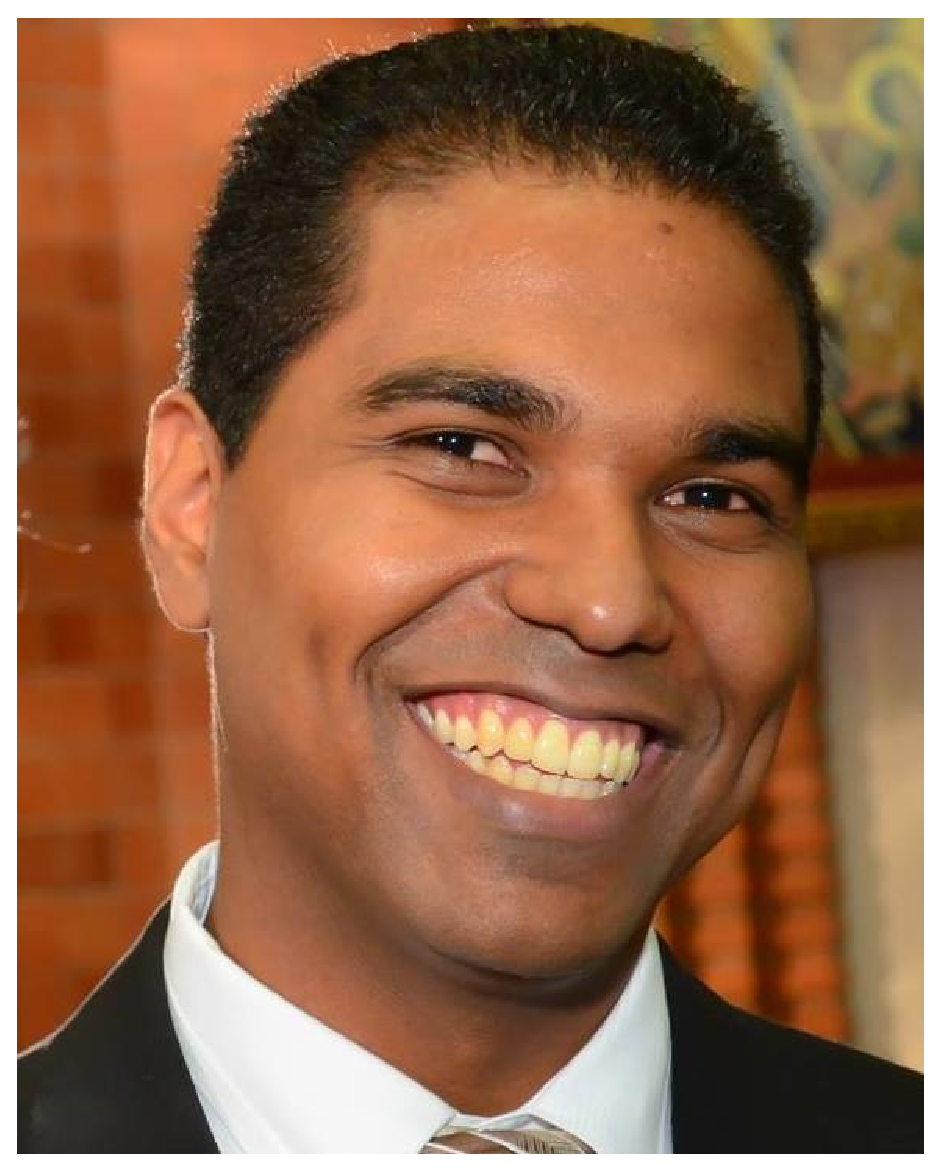
\includegraphics[width=1in,height=1.25in,clip,keepaspectratio]{Danilo_Lima.eps}}]{Danilo Alves de Lima}
received the B.S. degree in Control and Automation Engineering and M.S. degree in Electrical Engineering from Federal University of Minas Gerais (UFMG), Belo Horizonte, Brazil, in 2008 and 2010, and a Ph.D. degree in Information and Systems Technologies from the University of Technology of Compi\`{e}gne (UTC), Compi\`{e}gne, France, in 2015. Currently, he is an Associate Professor at the Engineering Department of the Federal University of Lavras (UFLA), Lavras, Brazil. 

He is a member of the Terrestrial Mobility Laboratory (LMT), UFLA, since 2015. He also worked with the Group for Research and Development of Autonomous Vehicles (PDVA), UFMG, and Heudiasyc UMR 7253, a common research laboratory between UTC and CNRS. His research interests include robotic navigation, intelligent vehicles development, and computer vision.
\end{IEEEbiography}
%
\begin{IEEEbiography}[{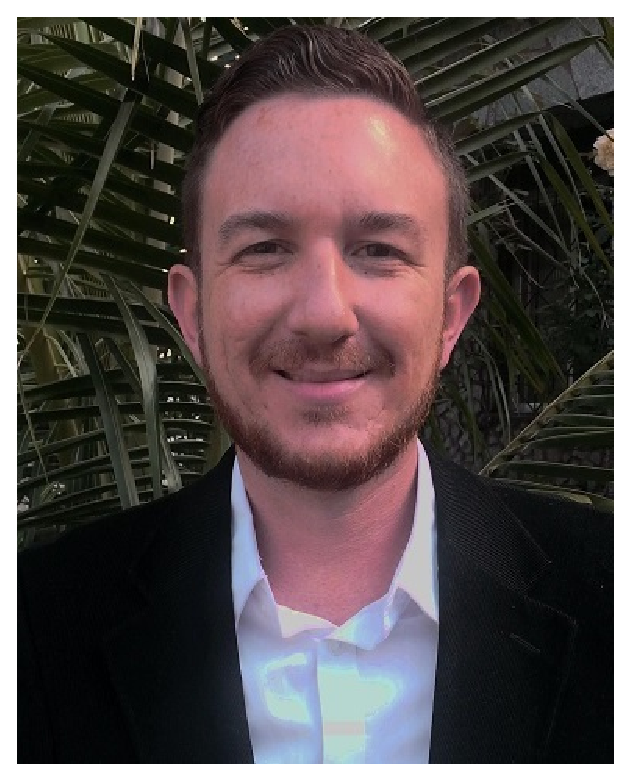
\includegraphics[width=1in,height=1.25in,clip,keepaspectratio]{Arthur_de_Miranda_Neto.eps}}]{Arthur de Miranda Neto}
received the B.S. degree in computer science - data processing - (1998). M.S. degree in mechanical engineering (2007) from State University of Campinas (UNICAMP), Campinas, Brazil, and a Ph.D. degree in information and systems technologies (2011) from the University of Technology of Compi\`egne (UTC), Compi\`egne, France, and in mechanical engineering from the UNICAMP, Brazil.

He was Officer (systems analyst) of the Brazilian Army between 1997 and 2005. He was Visiting Professor at the UNICAMP between 2012 and 2014. Since 2014, he is an Associate Professor in the Engineering Department at the Federal University of Lavras (UFLA) and head of the Terrestrial Mobility Laboratory (LMT). His research interests are in the field of robotic and mechatronic systems, more precisely in the area of automated driving systems.
\end{IEEEbiography}

\end{document}
